\section{Thesis Contributions}\label{sec:introduction:contributions}

In the following, we will detail the key contributions made by this dissertation.
We start with the core contribution, which addresses the \emph{principal \gls{RQ}}.

% \begin{large}
\begin{titled-frame}{\textbf{Core Contribution}}
% \noindent Safe Closed-form Control of Soft Robots with Learned Models
\noindent Safe and Precise Soft Robots via Closed-form Control with Learned Models
% compliant, stable, and efficient?
\end{titled-frame}
% \end{large}
% In this thesis, we devised two approaches for learning kinematic and dynamic models of soft robots that exhibit a physical structure, which we go into more detail about when discussing Contribution~\ref{contrib:learned_models}. As these learned models press well-defined kinetic and potential energy terms, we can leverage well-established feedback+feedforward control strategies originally developed for rigid manipulators~\citep{kelly1995tuning, kelly1996class, kelly1998global, sciavicco2012modelling}.
% Specifically, we combine a potential-shaping feedforward term~\citep{della2023model} with an integral-saturated PID~\citep{pustina2022p} as the feedback term. This control strategy allows us to exploit the learned model knowledge in the feedforward term while simultaneously rejecting disturbances and compensating modeling errors with the feedback term.
% Furthermore, instead of devising the controller via computationally expensive strategies such as \gls{RL} or \gls{MPC} as it typically needs to be done for learned models, the control input is available in closed form.
% Also, this strategy would allow us to inspect the stability of the closed-loop system and prove its stability using Lyapunov arguments~\citep{khalil2002nonlinear}, as we have already done for the open-loop system~\citep{stolzle2024input}.
% These stability guarantees enabled by the interpretability of the learned model are already one step towards ensuring \emph{safe control}. To advance and quantify the safety of soft robot control, we furthermore i) devise a safety metric that allows an analysis of the injury severity that could be caused by the closed-loop system and, particularly, establishing limits on the magnitude of the (proportional) feedback gains to meet the given safety requirements, and ii) develop stable high-level strategies for generating compliant motion behaviors by providing references/setpoints to the low-level controller.
In this thesis, we introduce two approaches for learning kinematic and dynamic models of soft robots that incorporate a physical structure (discussed in more detail under Contribution~\ref{contrib:learned_models}). Because these learned models encode well-defined kinetic and potential energy terms, we can leverage established error-based feedback+energy-shaping control strategies originally designed for rigid manipulators~\citep{kelly1995tuning, kelly1996class, kelly1998global, sciavicco2012modelling}. Specifically, we combine a potential-shaping feedforward term~\citep{della2023model} with an integral-saturated PID~\citep{pustina2022p} for feedback. This setup allows us to utilize the learned model within the feedforward component while still handling disturbances and compensating for modeling inaccuracies via the feedback term.
% 
Moreover, instead of relying on computationally expensive methods such as \gls{RL} or \gls{MPC}, which are often necessary for learned models, our controller provides a closed-form solution. This makes it possible to analyze the characteristics of the closed-loop system and formally prove stability using Lyapunov arguments~\citep{khalil2002nonlinear}, as already demonstrated for the open-loop case~\citep{stolzle2024input}. These stability guarantees—supported by the interpretability of the learned model—constitute an initial step toward \emph{safe control}.
% 
To further promote and quantify safety, we i) propose a safety metric that evaluates potential injury severity from the closed-loop system dynamics and specifically establishes bounds on the proportional feedback gains to ensure safety requirements and ii) develop stable high-level strategies to generate compliant motion behaviors by providing references/setpoints to the low-level controller.
Experimental verification of the contributions is an important aspect of this thesis, and we present some of the (soft) robot embodiments used in Fig.~\ref{fig:introduction:thesis_robots}.

This core contribution is enabled by multiple key contributions, which we detail in the following.

\begin{contribution}\label{contrib:safety_metric}
    A First Quantitative Safety Metric for Soft Robots
\end{contribution}
% In order to answer \gls{RQ}~\ref{rq:soft_robotic_safety}, we devise the first quantitative safety metric for soft robots in Chapter~\ref{chp:safetymetric}.
% To achieve this goal, we first investigate potential applications in the realm of design, control, and certification of such a safety metric. Subsequently, we state a list of requirements that a safety metric would need to (ideally) meet in order to be suitable for these applications.
% Finally, based on the existing, standardized criterion for collaborative robots~\citep{iso2016collaborative}, which considers the maximum contact experienced during a collision between a robot and human as a proxy for injury severity, we devise a quantitative safety metric that takes into account the particular characteristics of soft robots, such as dynamics that consider the continuous deformability of the backbone, elasticity, and contact anywhere along its body.
% The proposed safety metric comes in two flavors: the \gls{SRISC} models the injury severity for a given contact geometry, soft robot configuration, and velocity. The \gls{SRDHC} assess the safety of a soft robotic design under the given operating conditions, such as maximum velocity, maximum actuation torques, etc.
% Finally, we give recommendations for the safe design of soft robotic manipulators.
To address \gls{RQ}~\ref{rq:soft_robotic_safety}, we introduce the first quantitative safety metric for soft robots in Chapter~\ref{chp:safetymetric}. We begin by examining possible uses of such a metric in design, control, and certification. From there, we define a set of requirements that the metric should ideally satisfy to be suitable for these applications.
% 
Building on the existing, standardized criterion for collaborative robots~\citep{iso2016collaborative}—which uses maximum contact pressure during a collision with a human as a proxy for injury severity—we develop a metric that considers the distinctive features of soft robots, including their continuous deformability, elasticity, and the potential for contact along the entire robot body. The proposed safety metric has two variants: the \glspl{SRISC} models injury severity for a given contact geometry, robot configuration, and velocity, while the \glspl{SRDHC} assesses how safe a soft robotic design is under certain operating conditions (e.g., maximum velocity and actuation torques). 
% Finally, we provide recommendations for the safe design of soft robotic manipulators.

% This contribution demonstrates a pathway how in the future the safety of soft robots, and essential goal of this thesis, could be quantified, optimized, ensured via control, and certified.
% Furthermore, this contribution reveals the effect that controllers have on the safety of the closed-loop system - an often overlooked aspect in the domain of soft robots. Therefore, it informs us how we should design compliant controllers that do not compromise the safety of soft robots, by, for example, eliminating integral terms, and minimizing feedback gains, instead relying on an effective feedforward term that requires an accurate dynamical model of the soft robots. 
This contribution outlines a pathway for quantifying, optimizing, ensuring through control, and ultimately certifying the safety of soft robots—a central objective of this thesis. Moreover, it highlights the significant impact controllers have on the safety of the closed-loop system, an aspect often overlooked in soft robotics. Consequently, it guides us toward designing compliant controllers that maintain safety, for instance, by eliminating integral terms and minimizing feedback gains, while instead relying on effective feedforward strategies based on an accurate dynamic model of soft robots.

% \subsection{Leveraging Kinematic Models for Soft
% Robot Shape Sensing}
\begin{contribution}\label{contrib:kinematic_models_shape_sensing}
    Leveraging Kinematic Models for Soft Robot Shape Sensing    
\end{contribution}
% This contribution towards answering \gls{RQ}~\ref{rq:shape_sensing} enables more robust and accurate shape sensing for soft robots by exploiting existing kinematic model knowledge. This improved state estimation is required for the deployment of feedback controllers, and it thus directly contributes to the core contribution of this thesis.
% Below, we detail two approaches that make up this contribution.

% In the first, fully learning-free, method presented in Chapter~\ref{chp:srslam}, we leverage a monocular visual \gls{SLAM} algorithm to obtain multiple pose measurements distributed along the soft robotic backbone from camera images. Subsequently, we formulate an optimization problem that projects these samples of the soft robot's shape onto the kinematic model to obtain configuration estimates. This helps to limit the effects of estimation drift on the shape belief and ensures that we preserve consistency between the pose estimates and the kinematic model. 
% We verify the proposed algorithm both with a simulated \gls{CC} segment and on a real soft segment with an attached low-cost Raspberry Pi camera.
% A major benefit of this approach is that very good shape reconstruction performance is enabled by the combination of four already very established components: 1) low-cost monocular cameras, 2) \gls{vSLAM}, 3) the \gls{PCC}~\citep{webster2010design} kinematic model for soft robots, and 4) optimization based on the Levenberg-Marquardt algorithm~\citep{levenberg1944method, marquardt1963algorithm}.
% In the future, shape estimation performance could be (likely) very easily improved by, for example, replacing the used \gls{vSLAM} algorithm with the current \gls{SOTA} algorithm or by using more expressive kinematic parametrizations (e.g., \gls{GVS}~\citep{renda2020geometric}).

\begin{figure}[ht]
    \centering
    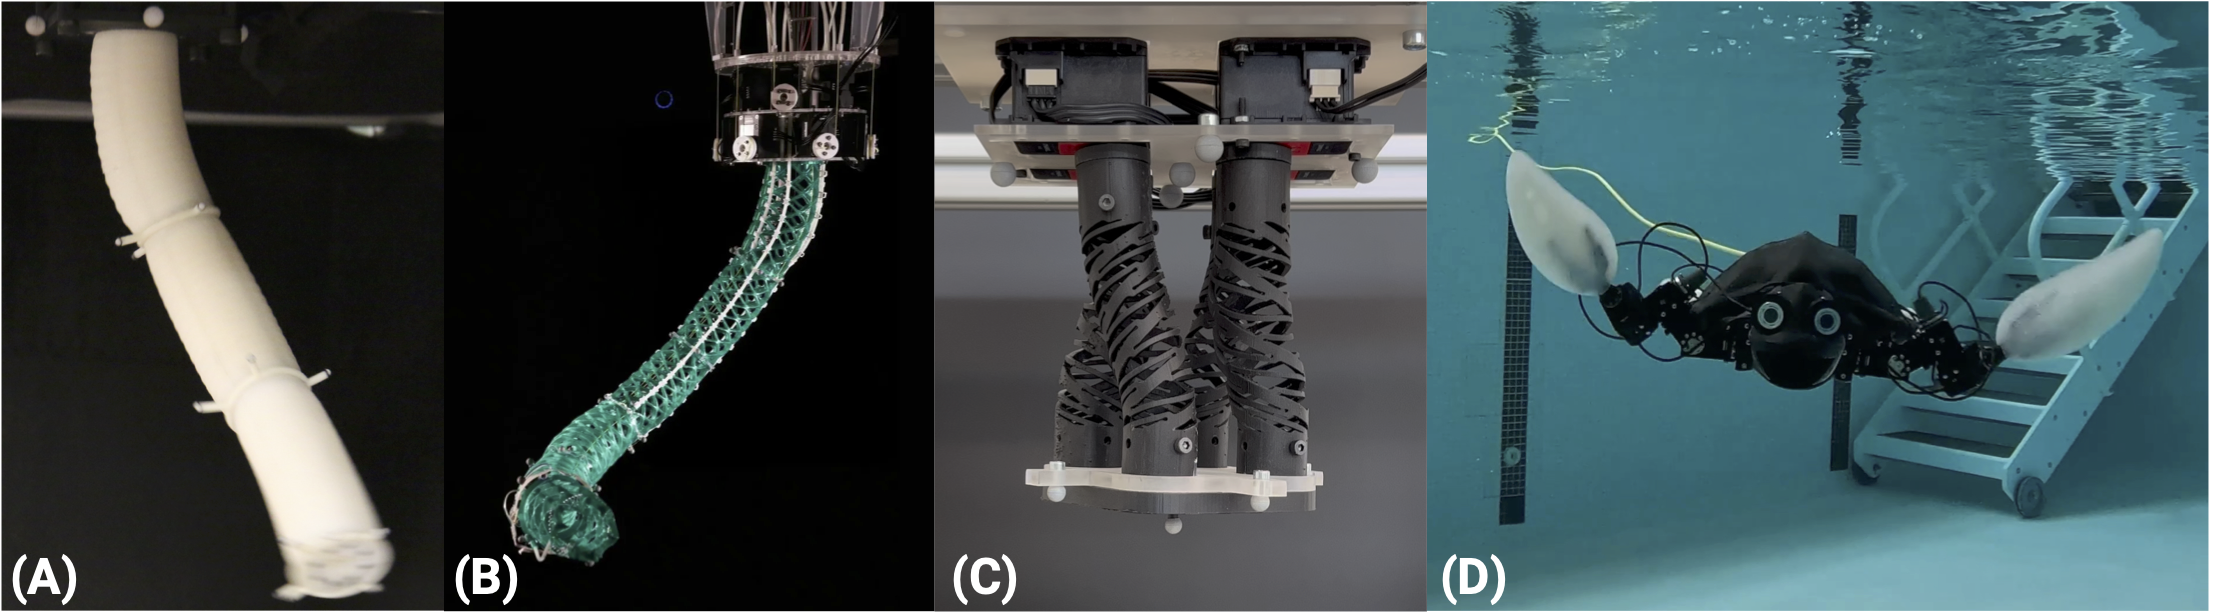
\includegraphics[width=1.0\linewidth]{introduction/figures/thesis_robots.pdf}
    \caption{
    Soft robot prototypes were used for experimental validation of the methods proposed in this thesis. 
    \textbf{Panel (A):} A three-segment pneumatic continuum soft robot made of silicon with three air cavities per segment. The picture is taken from ~\citet{katzschmann2019dynamic}.
    \textbf{Panel (B):} A tendon-driven continuum soft robot consisting of five segments based on a helicoid structure, coined Helix Robot~\citep{guan2023trimmed}.
    \textbf{Panel (C):} An \gls{HSA} soft robot based on 3D-printed auxetic metamaterials driven by four servo motors~\citep{lipton2018handedness, truby2021recipe}.
    \textbf{Panel (D):} A hybrid soft-rigid turtle robot combining a rigid body with limbs consisting of three servos and a rigid-soft flipper.
    }
    \label{fig:introduction:thesis_robots}
\end{figure}


% The second approach appears in Chapter~\ref{chp:promasens} and considers shape proprioception based on magnetic sensors. 
% Specifically, we propose to embed multiple magnets and magnetic sensors into 
% As magnetic fields in 3D can be very complex, a pure physics-based approach is not sufficient anymore. Therefore, we employ modern \gls{ML} approaches to aid us in the interpretation of the magnetic sensor readings. However, instead of learning the mapping from sensor readings to configuration estimates end-to-end, we leverage the kinematic model to simplify the learning problem and improve the data efficiency. Specifically, we use the kinematic model describing the backbone shape to parametrize the spatial relationship between a magnetic sensor and each magnet through a set of a few variables. 
% This then allows us to efficiently and robustly learn to predict the measurements of the magnetic sensor using a neural network. During inference, we then formulate an optimization problem that aims to estimate the soft robot shape by matching the actual and the predicted sensor measurements, which we solve through gradient descent.
% This approach demonstrates how existing prior knowledge, such as a kinematic model, can be used to reduce the size of the \emph{black-box}.

This contribution, which addresses \gls{RQ}~\ref{rq:shape_sensing}, improves the robustness and accuracy of shape sensing in soft robots by harnessing existing kinematic model knowledge.
% We accomplish this by solving nonlinear optimization problems that align the sensor measurements with the backbone shapes attainable by the kinematic model.
We achieve this by solving nonlinear optimization problems that align sensor measurements with the backbone shapes predicted by the kinematic model.
Enhanced state estimation is critical for deploying feedback controllers, thus directly supporting the thesis’s core contribution.
Below, we outline two distinct approaches.

The first method presented in Chapter~\ref{chp:srslam} combines monocular cameras embedded into the soft robot surveilling the environment with \gls{vSLAM} and a projection onto the kinematic model.
Specifically, the \gls{vSLAM} algorithm estimates multiple poses along the soft robot’s backbone based on the camera images. We then solve an optimization problem that projects these pose measurements onto the kinematic model, producing configuration estimates. This strategy mitigates estimation drift and preserves consistency between pose estimates and the kinematic model. We verify the algorithm both in simulation and on a real soft segment equipped with a low-cost Raspberry Pi camera. Its success stems from blending four well-established elements: (1) low-cost monocular cameras, (2) \gls{vSLAM}, (3) the \gls{PCC}~\citep{webster2010design} kinematic model, and (4) Levenberg-Marquardt optimization~\citep{levenberg1944method, marquardt1963algorithm}. Future work could further boost performance simply by, for example, using more advanced \gls{vSLAM} methods or more expressive kinematic parametrizations such as \gls{GVS}~\citep{renda2020geometric}.

The second method, included in Chapter~\ref{chp:promasens}, centers on shape proprioception with magnetic sensors. We embed multiple magnets and magnetic sensors in the robot, which yields complex 3D magnetic fields that are not sufficiently modeled by purely physics-based approaches. Consequently, we combine modern \gls{ML} techniques with a physics-based kinematic model rather than learning the entire sensor-to-configuration mapping in an end-to-end fashion. Specifically, the kinematic model represents the backbone shape and parameterizes the spatial relationship between each sensor and magnet using just a few variables. We then train a neural network to predict sensor readings based on these parameters. During inference, we solve an optimization problem via gradient descent that matches the actual sensor outputs to the model’s predictions, thereby recovering the robot’s shape. This approach illustrates how incorporating a known kinematic model reduces the size of the \emph{black-box} that needs to be learned in a data-driven approach.


\begin{contribution}\label{contrib:actuation_models}
    Soft Robot Control with Advanced Physics-Based Actuation Models
\end{contribution}
% We address \gls{RQ}~\ref{rq:actuation_models} by deriving advanced actuation models from first principles and subsequently leveraging them in model-based controllers by considering two cases, namely \gls{HSA} robots, and pneumatic piston-driven soft robots. We detail each case in the following paragraphs.
% \textcolor{orange}{How does this contribute to the core contribution?}

% \gls{HSA} robots~\citep{lipton2018handedness, chin2018compliant} consist of multiple (usually four) \gls{HSA} rods that are composed in a parallel fashion and connected at the tip. An elongation of the rods causes the robot to elongate and/or bend. However, instead of directly applying axial forces and rotational torques to infuse elongation and bending strains as it is usually done with most soft robot actuation techniques, these deformations are generated by the auxetic metamaterial of the \gls{HSA} rods: applying a torsional torque, for example by attaching an electric servo motor, at the base while constraining the tip causes the rods to twist which in turn is simultaneously transformed by the auxetic metamaterial into elongation of the rod.
% Furthermore, the applied torsional torques can cause the entire \gls{HSA} segment to twist, which is a rare deformation for soft robots.
% This complex actuation technique calls for the development of completely new, specifically actuation, models. However, while related work in recent years has proposed new designs~\citep{good2022expanding, good2025torque}, fabrication techniques~\citep{truby2021recipe}, proprioception algorithms~\citep{zhang2022vision}, and applications~\citep{chen2024real} for \gls{HSA} robots, accurate models~\citep{garg2022kinematic} and control concepts are still missing. In Chapters~\ref{chp:hsamodel} \& \ref{chp:hsacontrol}, we propose and experimentally verify several models and controllers for \gls{HSA} robots, respectively. In the following, we will introduce the contributions in more detail.
% In Chapter~\ref{chp:hsamodel}  of this thesis, we propose new kinematic, dynamic, and actuation models that are tailored to \gls{HSA} robots.
% First, we propose a novel kinematic parameterization, the \gls{SPCS} model, that is able to capture the 3D shape of \gls{HSA} rods with the least possible \gls{DOF}.
% For this purpose, we combine the existing \gls{CS} and \gls{PCS} models~\citep{renda2018discrete} and keep certain strains constant over the entire \gls{HSA} rod length while allowing other strains to vary in a piecewise constant fashion.
% Secondly, as existing work had already experimentally established that the mechanical characteristics, such as stiffness and rest length, of \gls{HSA} rods vary as a function of the actuation (i.e., the twist angle of the rod at the base), we develop a model that is able to capture this particular actuation characteristic and allows easy integration into existing dynamical models/simulators that are based on the \gls{DCM}.
% Thirdly, we implement the second contribution into an extension of PyElastica~\citep{naughton2021elastica} that is able to simulate the behavior of \gls{HSA} robots in 3D.
% Fourthly, we derive a kinematic parameterization based on the \gls{CS} model that accurately captures the deformation of planar \gls{HSA} robots with just three configuration variables. In this realm, we also state for the first time a closed-form solution for the inverse kinematics of a \gls{CS} robot.
% Fifthly, we devise a dynamical model for planar \gls{HSA} robots in Euler-Lagrangian form.
% Subsequently, we exploit in Chapter~\ref{chp:hsacontrol} the proposed models for control. Specifically, we propose two control approaches:
% Firstly, we devise a configuration-space P-satI-D+potential shaping regulator that combines an integral-saturated PID controller~\citep{pustina2022p} with compensation of steady-state forces at the desired setpoint, and that is able to move the end-effector of the planar \gls{HSA} robot towards a desired position in operational space.
% A core challenge here was to develop the necessary to make this more complex actuation model usable within the feedback+feedforward strategy. This, for example, required i) linearization of the actuation terms, 2) a mapping into actuation coordinates~\citep{pustina2024input}, and 3) solving the static inversion problem~\citep{della2025pushing}.
% Secondly, we propose and experimentally verify a operational space impedance controller that cancels the existing soft robot dynamics based on the model knowledge and allows the shaping of the stiffness field through a Cartesian-space PD feedback term. The key challenge here was a) to derive the operational-space dynamics of the \gls{HSA} robot~\citep{khatib1987unified, della2020model} and b) to map desired generalized torques into the underactuated control input.


% Pneumatic/fluidic actuation for soft robots is widely adopted for its fast response time and high and distributed forces/torques~\citep{marchese2015recipe, zaidi2021actuation}.
% While there exist several options for fluidic pressure supplies, such as rotary pumps or high-pressure supplies combined with valve-enabled pressure actuators, fluidic drive cylinders/pistons~\citep{marchese2014design, marchese2016design, parlikar2024concept, malas2024novel} have the advantages of i) a direction relationship between soft robot deformation and piston position and ii) a closed-volume system~\citep{marchese2016design}.
% However, there exists only relatively little research on modeling the behavior of such pneumatic piston-driven soft robots~\citep{marchese2014design, xavier2020modelling}.
% Furthermore, existing model-based soft robot controllers~\citep{della2020model, della2023model} do not take the dynamics of the actuator into account but instead rely on a cascaded control scheme where an outer loop running a (configuration-space) soft robot controller at approximately \SI{100}{Hz} passes pressure references to a faster inner PID-like controller regulating the piston at approximately \SI{1}{kHz}~\citep{marchese2014design}.
% However, this control scheme is only effective when the delay between the time when a pressure setpoint is set and finally reached is relatively small, which is only the case when either i) the electric drive of the piston is very powerful, fast,, and precise, and/or ii) the configuration/pressure setpoints vary relatively slowly.
% Consequently, either very performance, and with that, costly piston actuators are required, or the speed of the dynamic behavior of the soft robot is inherently limited.
% We aim to resolve these issues in Chapter~\ref{chp:backstepping} by modeling the potential energy stored in the fluidic as a function of the soft robot configuration and the piston positions. This allows us to formulate the coupled dynamics between the soft robotic and the piston system in Euler-Lagrangian form. Finally, we employ a backstepping approach~\citep{kokotovic1992joy, lozano1992adaptive, khalil2002nonlinear} to a nonlinear model-based feedback controller for the coupled system that exploits both the soft robot and the piston dynamics.

We address \gls{RQ}~\ref{rq:actuation_models} by deriving advanced actuation models from first principles and then embedding them in model-based controllers. Two case studies guide our work: \gls{HSA} robots and pneumatic piston-driven soft robots. These advanced actuation models feed into the thesis’s core contribution by informing us about the available physical priors for learning models.

\paragraph{HSA Robots.}
\glspl{HSA} robot~\citep{lipton2018handedness, chin2018compliant} typically feature several \gls{HSA} rods arranged in parallel and joined at the tip. Applying torsional torque at the base (e.g., via a servo motor) twists the rods, which in turn elongates and/or bends the robot through the rod’s auxetic metamaterial. This complex actuation mechanism can also induce twisting along the robot’s length, a rare deformation for soft robots. Despite ongoing research into new designs~\citep{good2022expanding, good2025torque}, fabrication processes~\citep{truby2021recipe}, and proprioception~\citep{zhang2022vision}, accurate models~\citep{garg2022kinematic} and control methods are lacking. In Chapters~\ref{chp:hsamodel} and \ref{chp:hsacontrol}, we propose and experimentally validate various models and controllers for \gls{HSA} robots.
%
Specifically, Chapter~\ref{chp:hsamodel} introduces a suite of kinematic, dynamic, and actuation models. First, we develop the \gls{SPCS} model to parameterize the 3D shape of \gls{HSA} rods minimally by fusing the \gls{CS} and \gls{PCS} approaches~\citep{renda2018discrete}. Next, we derive an actuation model that captures how the rod’s stiffness and rest length vary with twist angle, allowing us to integrate this phenomenon into existing \gls{DCM}-based simulators. We then implement our findings in a PyElastica~\citep{naughton2021elastica} extension, enabling 3D simulations of \gls{HSA} robots. For planar \gls{HSA} robots, we detail a simpler kinematic model based on \gls{CS}, culminating in a closed-form inverse kinematics solution. Finally, we present a dynamic model in Euler-Lagrange form suitable for planar \gls{HSA} manipulators.
%
Chapter~\ref{chp:hsacontrol} leverages these models to develop two control schemes. The first is a configuration-space P-satI-D plus potential-shaping regulator, integrating an integral-saturated PID controller~\citep{pustina2022p} with force compensation at the setpoint to guide the end-effector to a desired location in task space. 
% Such a control strategy of making a complex, underactuated, and non-affine control term more amendable for control could, in the future, also be important when devising closed-form controllers based on learned models - for example, when the latent space is higher-dimensional than the actuation space.
In the future, a strategy that renders a complex, underactuated, and non-affine control term more amenable to control may also prove valuable when developing closed-form controllers based on learned models—for instance, if the latent space exceeds the dimension of the actuation space.
The second is a operational space impedance controller that cancels the soft robot’s inherent dynamics and uses a Cartesian PD feedback term to shape the desired stiffness field. Key challenges include mapping generalized torques into the underactuated control input, linearizing actuation terms, and solving the static inversion problem~\citep{della2025pushing}.

\paragraph{Pneumatic Actuation Dynamics \& Backstepping Control.}
Pneumatic actuators are popular in soft robotics for their quick response and distributed force generation~\citep{marchese2015recipe, zaidi2021actuation}, with some variants employing fluidic pistons~\citep{marchese2014design, marchese2016design, parlikar2024concept, malas2024novel}. Such piston-driven actuation has at least two advantages: (1) the robot’s deformation is directly related to the piston position, and (2) they are closed fluid systems allowing easy use of the ideal gas law~\citep{marchese2016design}. However, relatively little work has been done on modeling these systems~\citep{marchese2014design, xavier2020modelling}, and existing controllers often adopt a cascaded approach that does not consider actuator dynamics, as a PID controller unaware of the soft robot dynamics is usually employed to control the piston. This is viable only if the fluidic system can quickly achieve pressure setpoints, necessitating high-performance (often costly) actuators or slow robot motions.
%
Chapter~\ref{chp:backstepping} addresses this limitation by modeling the potential energy stored in the fluid as a function of the robot’s configuration and the piston position, thereby coupling the piston and soft robot dynamics in Euler-Lagrange form. We then apply a backstepping approach~\citep{kokotovic1992joy, lozano1992adaptive, khalil2002nonlinear} to design a nonlinear, model-based feedback controller for the entire system, enabling tighter integration of actuator and robot dynamics.
In the future, such an actuation model could serve as a structural prior when learning models, such as learning the potential energy stored in the fluid analog to \glspl{LNN}~\citep{lutter2019deep}, therefore connecting to the core contribution. Furthermore, applying the backstepping procedure to a learned model appears to be an unexplored but interesting research avenue.

% \begin{contribution}
%     Techniques for Learning Soft Robot Models that Enable Stable Control in Closed-Form
% \end{contribution}

\begin{contribution}\label{contrib:learned_models}
    Integrating Physical Structure and Stability Guarantees into Learned Models
\end{contribution}
% In this thesis, we propose two approaches for learning control-oriented dynamical models of soft robots that expose the necessary (physical) structure to allow for closed-form control via energy shaping and stability analysis of the open- and closed-loop system via Lyapunov arguments~\citep{khalil2002nonlinear}, addressing \gls{RQ}~\ref{rq:physical_structure_learned_models}. We will detail both approaches in more detail below.
In this thesis, addressing \gls{RQ}~\ref{rq:physical_structure_learned_models}, we propose two approaches for learning control-oriented dynamical models of soft robots that incorporate the necessary (physical) structure to facilitate closed-form control through energy shaping, as well as stability analysis of both the open- and closed-loop systems using Lyapunov arguments~\citep{khalil2002nonlinear}.
% We achieve this by integrating physics-based dynamical models into the learning algorithm which determines the free parameters of the dynamics and optimally optimizes over a change of coordinates, such as an encoding into latent space.
% We outline the two approaches in detail below.
We achieve this by incorporating physics-based dynamical models into the learning algorithm, which then identifies the free parameters of the dynamics and optionally optimizes over a change of coordinates—such as encoding into latent space. We detail the two approaches below.

% In Chapter~\ref{chp:pcsregression}, we devise an algorithm that learns a soft robot strain model, specifically a \gls{PCS}-based model, directly from data of the shape evolution of the soft robot's backbone.
% While \gls{PCS}~\citep{renda2018discrete} and similar kinematic parameterizations are already very much established in the literature, their design requires much expert knowledge and/or trial-and-error. For example, the modeling engineer needs to determine the number of segments, the length of each segment, and the active strains for each segment.
% Finally, the dynamic system parameters identification procedure via nonlinear optimization can be computationally quite demanding and possibly badly conditioned. 
% Instead, our proposed approach, composed of two algorithms, can directly identify all necessary parameters from the evolution of pose samples approximating the soft robot's shape.
% The first algorithm identifies a suitable kinematic parametrization, including the number of segments and their lengths, using an iterative procedure by analyzing the strain progression along the backbone. 
% The second algorithm subsequently derives the physics-based dynamical model from first principles based on the previously identified kinematic parametrization and represents the Euler-Lagrangian dynamic using a a sum of basis functions. This allows the dynamic parameters to be identified in closed form using linear least-squares. Additionally, the algorithm leverages heuristics, such as the identified strain stiffness, to neglect certain strains and, thus, iteratively reduce the \gls{DOF} of the model, making it more efficient and suitable for control.
% We verify the proposed approach in simulation and benchmark the performance at predicting the future evolution of the soft robot over long horizons against \gls{SOTA} \gls{ML} approaches such as \glspl{RNN}, \glspl{NODE}, etc.
In Chapter~\ref{chp:pcsregression}, we introduce an algorithm designed to learn a soft robot strain model, specifically a \gls{PCS}-based model, directly from data representing the shape evolution of the soft robot’s backbone.
Although \gls{PCS}~\citep{renda2018discrete} and similar kinematic parametrizations~\citep{alessi2024rod} are well-established in the literature, their design often requires significant expert knowledge and/or trial-and-error. For instance, the modeling engineer must determine the number of segments, the length of each segment, and the active strains for each segment.
Additionally, identifying dynamic system parameters through nonlinear optimization can be computationally intensive and potentially ill-conditioned.
Our proposed approach, comprising two algorithms, circumvents these challenges by directly identifying all necessary parameters from pose samples approximating the soft robot’s shape evolution.
The first algorithm uses an iterative procedure to determine an appropriate kinematic parameterization, including the number and length of the segments, by analyzing the strain progression along the backbone.
The second algorithm then derives a physics-based dynamical model from first principles using the previously identified kinematic parameterization, representing the Euler-Lagrangian dynamics as a sum of basis functions. This enables dynamic parameter identification in closed form through linear least-squares.
Additionally, the algorithm employs heuristics, such as identified strain stiffness, to neglect certain strains, iteratively reducing the \gls{DOF} of the model, thereby improving efficiency and control suitability.
We validate the proposed approach through simulations and benchmark its performance in predicting the soft robot’s future shape evolution over long horizons against \gls{SOTA} \gls{ML} methods, including \glspl{RNN}, \glspl{NODE}, and others.

The second approach, presented in Chapter~\ref{chp:con}, considers the problem setting of learning the dynamics of physical systems, and specifically, of continuum soft robots from high-dimensional observations, such as sequences of images.
As learning the dynamics directly in image space is considered to be intractable, an established procedure is to employ an autoencoder, such as a \gls{VAE}~\citep{kingma2014auto}, and then learning the dynamics of a lower dimensional space, referred to as the latent space.
Contrary to existing literature, which mostly uses \glspl{MLP}, \glspl{RNN} or \glspl{NODE}, we propose to learn the latent dynamics with a network of coupled oscillators that consists of damped harmonic oscillators that are connected by a nonlinear potential.
Crucially, this now allows us to assign a mechanical interpretation to each latent variable - the position of one of the harmonic oscillators.
Furthermore, the physical structure of the \glsxtrfull{CON} dynamics, in particular the network's energy terms, allow us to derive very strong stability guarantees, such as \glsxtrfull{GAS} for the unactuated and \glsxtrfull{ISS} for the actuated latent dynamical system, using Lyapunov arguments~\citep{khalil2002nonlinear}.
Finally, we propose an approximated closed-form solution to the rollout of the \gls{CON} dynamics that enables a speed-up of both training and inference.
We benchmark the proposed approach against \gls{SOTA} \gls{ML} approaches extensively on rendered image sequences of various simulated systems, including different simulated soft robots.


\begin{contribution}\label{contrib:model_based_control_with_learned_models}
    Exploiting Learned Models for Closed-Form Model-Based Control
\end{contribution}
% Also contributing to ~\gls{RQ}~\ref{rq:physical_structure_learned_models} and building on Contribution~\ref{contrib:model_based_control_with_learned_models}, we devised in this a strategy for closed-form regulation based on learned models.
% Here, we build on the seminal work that devised feedback+feedforward controllers for rigid manipulators~\citep{kelly1996class, kelly1997pd, kelly1998global, sciavicco2012modelling}, later extended to the physics-based model control of soft robots by accounting for linear elastic forces~\citep{della2020model, della2023model} and nonlinear elastic forces demonstrated in Chapter~\ref{chp:hsacontrol}.
% As the feedback term, we employ a P-satI-D~\citep{pustina2022p} that, compared to PD+ controllers~\citep{della2020model}, has an improved ability to compensate for model errors through the integral action while its saturation helps to decrease the likelihood of instability~\citep{pustina2022p}.
% An important underlying assumption, similar to fully physics-based models, is that we require the state space to be continuous. This means that special techniques~\citep{maithripala2015intrinsic} are required to deal with other geometric spaces, such as Lie groups, which do not directly fulfill this property.
% As the feedforward term, we choose to compensate the potential forces at the desired robot state, which requires the potential field to be (locally) convex~\citep{della2023model} in order that we need to rely on the integral action as little as possible. This strategy can be intuitively interpreted such that we reshape the potential energy of the closed-loop system to exhibit its (local) minimum at the setpoint.
% The result is a very simple but effective control strategy.
% Having already employed this P-satI-D+potential shaping control strategy on the entirely physics-based \gls{HSA} model as part of Contribution~\ref{contrib:actuation_models}, we verify additionally in simulation for both the learned strain-based model in Chapter~\ref{chp:pcsregression} and for latent space control based on \gls{CON} dynamics in Chapter~\ref{chp:con}.
Additionally contributing to \gls{RQ}\ref{rq:physical_structure_learned_models} and building on Contribution~\ref{contrib:model_based_control_with_learned_models}, we here propose a closed-form regulation strategy based on learned models. In doing so, we draw on seminal work that introduced closed-form model-based controllers for rigid manipulators~\citep{kelly1996class, kelly1997pd, kelly1998global, sciavicco2012modelling}, subsequently adapted for the physics-based control of soft robots by considering both linear~\citep{della2020model, della2023model} and, as shown in Chapter~\ref{chp:hsacontrol}, nonlinear elastic forces~\citep{borja2022energy}.
The controller combines an integral-saturated PID (P-satI-D)~\citep{pustina2022p} with an energy-shaping feedforward term. We motivate the considerations behind this strategy in the following.

For the error-based feedback component, we use a P-satI-D controller~\citep{pustina2022p}, which offers stronger robustness against modeling errors via its integral action while saturation reduces the risk of instability~\citep{pustina2022p}. Compared to PD feedback laws~\citep{della2020model}, this approach is more effective at mitigating unmodeled or wrongly modeled dynamics.
%
A key assumption—akin to purely physics-based models—is that the state space must be continuous. Consequently, specialized methods~\citep{maithripala2015intrinsic} are necessary for other geometric spaces (e.g., Lie groups), where continuity in this sense does not hold directly.

For the feedforward portion, we compensate the potential forces at the target state, requiring the potential field to be (locally) convex~\citep{borja2022energy, della2023model}. The aim is to rely on the integral action as little as possible, effectively reshaping the closed-loop system’s potential energy so its (local) minimum is at the desired setpoint. 
% Furthermore, the goal needs to be reachable by the control, which means that the setpoint is a reachable equilibrium of the closed-loop system. 
% In the underactuation, it is additionally important for the null-dynamics to be asymptotically stable in order to obtain a stable control behavior~\citep{borja2022energy}.
Additionally, the control must be able to reach the goal, which requires the setpoint to be a reachable equilibrium of the closed-loop system. In the underactuated case, it is also crucial for the null dynamics to be asymptotically stable in order to guarantee a stable control response~\citep{borja2022energy}.
% The benefit of compensating the dynamics (specifically, here, the static forces) at the target state instead of canceling the dynamics at the current state is increased robustness against mismatches between the (learned) model and the actual dynamics as unmodeled dynamics are less likely to become dominant.
Compensating for the dynamics—specifically the static forces—at the target state, rather than canceling them at the current state, enhances robustness against mismatches between the learned model and the actual dynamics, as unmodeled dynamics are less likely to dominate in the closed-loop system.

This combination of integral-saturated PID feedback action and potential shaping feedforward action yields a straightforward yet powerful control approach.
%
Having already applied this P-satI-D+potential shaping strategy to a fully physics-based \gls{HSA} model as part of Contribution~\ref{contrib:actuation_models}, we further validate it in simulation with the learned strain-based model in Chapter~\ref{chp:pcsregression} and for latent space control using \gls{CON} dynamics in Chapter~\ref{chp:con}.


\begin{contribution}\label{contrib:motion_behaviors}
    Beyond Low-Level Control: Generating Compliant Motion Behaviors for Soft Robots
\end{contribution}

% We contribute towards \gls{RQ}~\ref{rq:compliant_motion_behaviors} by proposing two approaches that generate compliant motion behavior for soft robots: First, we present Chapter~\ref{chp:braincontrol} a \gls{BMI} approach for guiding a low-level impedance control with motor imagery based on measurements by a wearable \gls{EEG} device. Second, we show in Chapter~\ref{chp:osmp} how a neural motion policy parametrized by a learned dynamical system with stability guarantees can be used for learning complex motion behaviors from demonstration can be used as a reference provider for a low-level soft robot controller. 
% \gls{RQ}~\ref{rq:compliant_motion_behaviors} ensures that not the safety enabled by the soft robot's body and compliant low-level controller is not jeopardized by the high-level motion behavior.
% In the following two paragraphs, we will introduce both lines of research in more detail.

% \glspl{BMI} promise barrier-free and physical-interaction-free operation of machines, and specifically robots, by analyzing the neural activity of the user and are particularly an interesting choice for allowing robots to assist impaired or elderly people with \gls{ADL}.
% However, currently, the classification of motor imagery from few-channel, wearable EEG devices exhibits relatively low accuracy for more than two classes~\citep{arpaia2022non, lee2024noir}. This can cause significant safety concerns when operating high-inertia, fast-moving, rigid robots using motor imagery. Therefore, soft robots, with their passive compliance, seem like a promising avenue as they would allow errors in the \gls{BMI} to occur without jeopardizing safety.
% Despite this promise, guiding soft robotic manipulators with \glsxtrfull{BMI} has not yet been explored in literature.
% In Chapter~\ref{chp:braincontrol}, we develop a \gls{BCI} protocol that allows users, for the first time, to operate soft robotic manipulators by imagining motor movements.
% As an \gls{EEG} device, we use a wearable cap with three channels, which promises in the future to take the operation with brain signals out of stationary lab environments.
% As achieving (relatively) high classification accuracies of the motor imagery using \gls{LDA} is currently only feasible on binary classification accuracies, an emphasis of the research was to identify a protocol that allows binary classifications to precisely and robustly control the movement of the soft robot end-effector in a plane.
% We achieve this by running two classifiers in parallel, one of which switches the coordinate axis of motion based on the classification of yaw clinching and another that controls the direction of motion (i.e., positive or negative sign) along the active coordinate axis by classifying motor imagery. 
% We experimentally verify the proposed \gls{BMI} protocol with a planar \gls{HSA} robot by relaying the operational space references generated by the \gls{BMI} system as setpoints/attractors to the compliant impedance controller developed as part of Contribution~\ref{contrib:actuation_models}.
% We quantitatively evaluate the brain signal-guided \emph{control} by visually projecting operational space goals stemming from the sequence of step functions onto a screen behind the \gls{HSA} robot.
% The operator then aims to guide the soft robot's end-effector toward the goal as fast as possible with motor imagery.
% We benchmark the \gls{BMI} interface against i) a very established \gls{HCI} - a keyboard, and ii) the low-level impedance controller directly having access to the goals, which we consider to be privileged information in this case.
% Finally, we also tackle the problem setting of assisting humans with a simple \glsxtrfull{ADL} by guiding the end-effector of a \gls{HSA} robot with brain signals to release hairspray from a bottle, which showcases the compliance and intelligence of the integrated system consisting of body, low-level motor control, and motion guided by the \gls{BMI} system.

% \glsxtrfull{DMP} parameterize motion policies with dynamical systems~\citep{ijspeert2013dynamical, saveriano2023dynamic} and allow for efficient learning of complex motions from demonstration (e.g., kinesthetic teaching, biomimetics, teleoperation, etc.).
% Particularly interesting is the case where the dynamic system does not exhibit an explicit dependence on time, as this allows for natural and compliant behavior even under perturbation~\citep{ijspeert2013dynamical}.
% However, the use of \glspl{DMP} within the realm of soft robotic manipulators has not yet been investigated.
% In Chapter~\ref{chp:osmp}, we propose an approach that can learn periodic motions from demonstration and track these demonstrations in a provably stable and compliant fashion without a time dependence.
% We accomplish this by building on the trailblazing literature on \glsxtrfull{SMP}~\citep{ijspeert2013dynamical, rana2020euclideanizing, perez2023stable} and propose a new approach that combines a bijective encoder with latent dynamics governed by a supercritical Hopf bifurcation. The \emph{simple} formulation of the latent dynamics allows us to prove their stability easily, and the expressiveness and diffeomorphism enabled by the Euclideanizing flows~\citep{dinh2016density, rana2020euclideanizing} allows us to learn complex motions while giving us the ability transfer these stability guarantees back into the space where the demonstration was provided.
% In practice, we map the current position of the robot in oracle space into latent space where we evaluate the \nth{1} order dynamics of the Hopf bifurcation, providing us with a latent velocity.
% Subsequently, we evaluate the (analytical) inverse Jacobian of the encoder to map the latent velocity into a desired velocity in oracle space, which would serve as a reference for the low-level motor controller of the system.
% We extensively validate this approach experimentally on a helicoid soft robot~\citep{guan2023trimmed}, a turtle robot swimming in a pool, a UR5 manipulator cleaning a whiteboard, and a Kuka \gls{Cobot} in human-contact-rich scenarios.
% The presented approach serves as an example of how compliant and natural motion policies for soft robots can be effectively learned from demonstrations of complex behavior.

Turning to \gls{RQ}~\ref{rq:compliant_motion_behaviors}, we propose two methods for generating compliant soft robot motion at a higher control level. Chapter~\ref{chp:braincontrol} covers a \gls{BMI}-based protocol that uses wearable \gls{EEG} to supply references to a low-level impedance controller, while Chapter~\ref{chp:osmp} focuses on learning motion policies from demonstration via a dynamical system. These strategies ensure that high-level policies do not undermine the inherent safety offered by the soft robot body and compliant low-level controllers.

\paragraph{Guiding Soft Robots via Motor Imagery.}
\glspl{BMI} allow users to operate machines through neural signals—particularly appealing for assisting individuals with limited mobility. Yet classification accuracies for motor imagery on wearable EEG devices are low for more than two classes~\citep{arpaia2022non, lee2024noir}, raising safety issues if used with fast, high-inertia rigid robots. Soft robots, by contrast, offer a passive compliance that can reduce risks from erroneous \gls{BMI} commands. However, controlling soft robots with \gls{BMI} has not yet been explored.
%
In Chapter~\ref{chp:braincontrol}, we introduce a brain-computer interface protocol that, for the first time, lets users operate a soft robotic manipulator using motor imagery. We employ a wearable, three-channel \gls{EEG} cap, aiming to in the future transition brain-controlled manipulations beyond traditional lab settings. Since robust motor imagery classification beyond two classes remains challenging, we devised an effective protocol that combines two parallel binary classifiers: one to select the active coordinate axis (based on yaw clinching) and another to determine movement direction along this axis (based on motor imagery). We validate our approach on a planar \gls{HSA} robot, where the \gls{BMI}-derived commands serve as setpoints for a compliant impedance controller (developed in Contribution~\ref{contrib:actuation_models}).
% We quantitatively evaluate the brain signal-guided \emph{control} by visually projecting operational space goals stemming from the sequence of step functions onto a screen behind the \gls{HSA} robot.
In a quantitative evaluation of the brain signal-driven control, we visually project step-function-based operational space goals onto a screen behind the \gls{HSA} robot.
% 
For benchmarking, we compare this \gls{BMI} system against (1) a keyboard interface and (2) a privileged scenario where the low-level controller has direct access to goal positions. Additionally, we show how this scheme can assist with a real-world \gls{ADL} task—guiding the robot’s end-effector with brain signals to spray hairspray—highlighting the synergy between the soft robot’s compliance, a suitable low-level controller, and higher-level \gls{BMI}-based commands.

\paragraph{Learning Stable Period Motions from Demonstration.}
\glspl{DMP} represent a well-known framework for learning complex motions from demonstrations~\citep{ijspeert2013dynamical, saveriano2023dynamic}. In soft robotics, adopting time-invariant \glspl{DMP} is particularly appealing for ensuring compliance under perturbations~\citep{ijspeert2013dynamical}, yet this approach remains unexplored. In Chapter~\ref{chp:osmp}, we present a method for learning periodic motions from demonstrations and reproducing them in a provably stable and compliant manner—without explicit time dependence.
% 
Our framework extends \glsxtrfull{SMP}~\citep{ijspeert2013dynamical, rana2020euclideanizing, perez2023stable} by combining a bijective encoder with latent dynamics governed by a supercritical Hopf bifurcation. The Hopf system’s simple latent dynamics facilitate stability proofs, while the diffeomorphism introduced by Euclideanizing flows~\citep{dinh2016density, rana2020euclideanizing} enables us to learn complex motions and transfer stability guarantees back to the original demonstration space. Practically, we encode the robot’s current position into the latent space, evaluate the Hopf system to obtain a latent velocity, and then map that velocity back to the demonstration space via the encoder’s analytical inverse Jacobian—yielding a velocity reference for a low-level motor controller, such as the configuration or operational space controllers presented in Chapter~\ref{chp:hsacontrol}.
% 
We conduct extensive experiments with diverse systems: a helicoid soft robot~\citep{guan2023trimmed}, a swimming turtle robot, a UR5 manipulator for whiteboard cleaning, and a Kuka \gls{Cobot} for tasks involving human contact. The results demonstrate that our approach can learn intricate motion patterns while preserving compliance, making it a promising path forward for soft robot motion planning.